\newpage
\section{图的基本概念}
\subsection{图和简单图}
\subsubsection{图的定义及其相关概念}

\noindent 图的定义:
\begin{definition}
	一个图$G$定义为一个有序对$<V,E>$,记为$G=(V,E)$,其中:
	\begin{enumerate}
		\item $V$是一个有限的非空集合,称为顶点集合,其元素称
		为顶点或点. 用$|V|$表示顶点数;
		\item $E$是由$V$中的点组成的无序对构成的集合,称为边集,
		其元素称为边,且同一点对在$E$中可以重复出现多次.用
		$|E|$表示边数.
	\end{enumerate}
\end{definition}

\noindent 图的相关概念:
\begin{enumerate}
	\item \textcolor{red}{有限图}:顶点集和边集都有限的图称为有限图。
	\begin{note}
		无限图也是大量存在的!如正整数集合上的“整除关系”
	图就是一个无限图。但我们课程只涉及“有限图”.
	\end{note}
	\item \textcolor{red}{平凡图与空图}:只有一个顶点的图称为平凡图;只有点
	没有边的图称为空图.
	\item \textcolor{red}{n阶图}:顶点数为n的图,称为n阶图.
	\item \textcolor{red}{(n, m) 图}:顶点数为n的图,边数为m的图称为(n, m) 图.
	\item \textcolor{red}{边的重数}:连接两个相同顶点的边的条数称为边的重
	数;重数大于1的边称为重边.
	\item \textcolor{red}{环}:端点重合为一点的边称为环
	\item \textcolor{red}{简单图}:无环无重边的图称为简单图;其余的图称为复合图.
	\item \textcolor{red}{顶点u与v相邻接}:顶点u与v间有边相连接(u adjv);其中
	u与v称为该边的两个端点.
		\begin{note}
		规定一个顶点与自身是邻接的.
		\end{note}
	\item \textcolor{red}{顶点u与边e相关联}:顶点u是边e的端点.
	\item \textcolor{red}{边e1与边e2相邻接}:边e1与边e2相邻接:边e1与边e2有公共端点.
\end{enumerate}

\subsubsection{图的同构}
\noindent 图的同构:\colorbox{yellow}{\textcolor{red}{如果顶点数相同、边数相同的
		两个图,其结构形式也相同}},那么这两个图同构.
\begin{definition}
	设有两个图 \( G_{1}=\left(V_{1}, E_{1}\right) \) 和 \( G_{2}=\left(V_{2}, E_{2}\right) \), 若在其顶点 集合间存在双射, 使得边之间存在如下关系: \( \mathbf{u}_{1}, \mathbf{v}_{1} \in \mathbf{V}_{1} \),
	\( \mathbf{u}_{2}, \mathbf{v}_{2} \in \mathbf{V}_{2} \), 设 \( \mathbf{u}_{1} \leftrightarrow \mathbf{u}_{2}, \mathbf{v}_{1} \leftrightarrow \mathbf{v}_{2} ; \mathbf{u}_{1} \mathbf{v}_{1} \in \mathbf{E}_{1} \) 当且仅当 \( \mathbf{u}_{2} \mathbf{v}_{2} \in \mathbf{E}_{\mathbf{2}} \), 且 \( u_{1} v_{1} \) 与 \( u_{2} v_{2} \) 的重数相同。称 \( G_{1} \) 与 \( G_{2} \) 同构, 记为:
	\[
	G_{1} \cong G_{2}
	\]
\end{definition}
\begin{note}
	\begin{itemize}
	\item 图同构的两个必要条件: \colorbox{yellow}{\textcolor{red}{顶点数相同;边数相同.}}
	\item 研究图的同构问题,核心是同构的判定问题.
	\item 3(4)个顶点非同构简单图有 4(11)个
	\end{itemize}
\end{note}

\subsubsection{完全图、偶图与补图}
\noindent {\bfseries \textcolor{ecolor}{完全图:}}
\begin{enumerate}
	\item \colorbox{yellow}{\textcolor{red}{完全图}}:完全图是一个简单图,且任意一个
		顶点都与其它每个顶点有且只有一条边相连接.
	\item \colorbox{yellow}{\textcolor{red}{n阶完全图}}: n个顶点的完全图用$K_n$表示.
	\item $K_n$的边数:
		\[
		\colorbox{yellow}{$m(K_n)=\dfrac{1}{2}n(n-1)$}
		\]
\end{enumerate}

\noindent {\bfseries \textcolor{ecolor}{偶图:}}

\noindent 偶图的特征:顶点分成不相交的两部分;任意一条边两个端点分属于两部分顶点.
\begin{definition}[偶图]
	所谓具有二分类$({X}, {Y})$的偶图(或二部图)是指一
	个图,它的点集可以分解为两个(非空)子集${X}$和${Y}$,使得每条
	边的一个端点在$X$中,另一个端点在$Y$中.
\end{definition}
\begin{note}
	\textcolor{red}{偶图不能有环,不能有三角形,可以有重边}
\end{note}


\begin{definition}[完全偶图]
完全偶图是指具有二分类 \( ({X}, {Y}) \) 的简单偶图, 其中 \( {X} \) 的每个顶点与 \( {Y} \) 的每个顶点相连, 若 \( |X|=n_{1},|Y|=n_{2} \), 则这 样的偶图记为 \colorbox{yellow}{\( K_{n_1, n_2} \)}.
\end{definition}

\begin{note}
	完全偶图是完全二部图. \textcolor{red}{偶图可以是只有两个点的空图,即偶图可能没有边}.
\end{note}

\noindent {\bfseries \textcolor{ecolor}{简单图的补图:}}
\begin{definition}[补图]
	对于一个简单图$G=(V,E)$,令集合
	\[
	E_1=\{uv|u\ne v, u, \in V  \}
	\]
	则称图$H=(V,E_1\textbackslash E)$为$G$的补图,记作$H=\overline{G}.$
\end{definition}
\begin{note}
	\begin{itemize}
		\item 只有简单图才能定义补图;
		\item n阶简单图和其补图的顶点集合是相同的;
		\item n阶简单图任意一对顶点邻接的充分必要条件是这对顶点在其补图中不邻接;
		\item n阶简单图的边数与其补图的边数之和等于$K_n$的边数;
		\item 补图是经常涉及的概念,在图结构分析中有重要的作用。	
	\end{itemize}
\end{note}

\begin{definition}[自补图]
	如果图$G$与其补图同构,则称$G$为自补图。
\end{definition}
\begin{note}
	\textcolor{red}{并不是任意一个简单图都是自补图.}
\end{note}


\begin{theorem}
	若n阶图是G的自补图,则有:\colorbox{yellow}{$n\equiv 0, 1(\mathrm{mod 4})$}.
\end{theorem}
\begin{proof}
	n阶图是G的自补图,则有
	\colorbox{yellow}{$m(G) +m(\overline{G}) = m(K_n) = \dfrac{1}{2}n(n-1)$}
	
	且\colorbox{yellow}{$m(G) =m(\overline{G})$}
	
	所以\colorbox{yellow}{$m(G) = \dfrac{1}{4}n(n-1)$}.因为$n$是正整数,所以:\colorbox{yellow}{$n\equiv 0, 1(\mathrm{mod 4})$}.
\end{proof}

\subsubsection{顶点的度和图的度序列}
\noindent {\bfseries \textcolor{ecolor}{顶点的度及其性质:}}
\begin{definition}[顶点的度]
$G$的顶点$v$的度$d(v)$是指$G$中与$v$关联的边的数
目,\textcolor{red}{每个环计算两次}.
\end{definition}
\begin{note}
	\begin{itemize}
		\item 分别用$\delta(G)$和$\varDelta(G)$表示图$G$的最小与最大度.
		\item 奇数度的顶点称为奇点,偶数度的顶点称偶点.
		\item \colorbox{yellow}{\textcolor{red}{$k$-正则图}}:设$G = (V, E)$为简单图,如果对所有$v\in V$,有$d(v) = k$,称图$G$为$k$-正则图,其边数和点数满足\colorbox{yellow}{$3n=2m$}.
	\end{itemize}
\end{note}

\begin{theorem}[握手定理]
	图$G=(V, E)$中所有顶点的度的和等于边数$m$的
	2倍,即:
	\[
	\colorbox{yellow}{$\sum\limits_{v\in V(G)} d(v)= 2m$}
	\]
\end{theorem}
\begin{proof}
	由顶点度的定义知:图中每条边给图的总
	度数贡献2度,所以,总度数等于边数2倍.
\end{proof}
\begin{corollary}
	在任何图中,奇点个数为偶数.
\end{corollary}
\begin{proof}
	设$V_1,V_2$分别是$G$中奇点集和偶点集.则由
	握手定理有:
	\[
	\sum\limits_{v\in V_1}d(v) + \sum\limits_{v\in V_2}d(v)= \sum\limits_{v\in V}d(v)=2m
	\]
	是偶数。由于上式左边第二项是偶数, 所以左边第一
	项是偶数,于是奇度点个数必为偶数。
\end{proof}

\begin{corollary}
	正则图的阶数和度数不同时为奇数.
\end{corollary}
\begin{proof}
设$G$是$k$-正则图,若$k$为奇数,则由上一个推论知正则图$G$的点数必为偶数
\end{proof}

\begin{corollary}
	$\delta$和$\varDelta$表示图$G$的最小与最大度,则
	\[
	\colorbox{yellow}{$\delta \leq \dfrac{2m}{n} \leq \varDelta$}
	\]
\end{corollary}
\begin{proof}
	由握手定理有
	\[
	\colorbox{yellow}{$n\delta \leq \sum\limits_{v\in V(G)} d(v)= 2m\leq n\varDelta$}
	\]
	所以,\colorbox{yellow}{$\delta \leq \dfrac{2m}{n} \leq \varDelta$}
\end{proof}


\noindent {\bfseries \textcolor{ecolor}{图的度序列及其性质:}}
\begin{definition}[度序列]
一个图$G$的各个点的度$d_1, d_2 , \cdots , d_n$构成的非负整数组
$(d_1, d_2,\cdots , d_n)$称为$G$的度序列
\end{definition}
\begin{note}
	\begin{itemize}
		\item 一个图的度序列与序列中元素排列无关;
		\item 给定一个图,只对应唯一一个度序列;
		\item 同构的图具有相同的度序列.
	\end{itemize}
\end{note}
\begin{theorem}
	非负整数组$(d_1, d_2, \cdots, d_n)$是图的度序列的充分必
	要条件是序列中元素总和为偶数.
\end{theorem}
\begin{proof}
\noindent 必要性:由握手定理立即得到

\noindent 充分性:如果$\sum\limits_{i=1}^{N} d_i$为偶数,则数组中为奇数的数字个数必为偶数 
\end{proof}

\noindent \textcolor{red}{根据度序列画图(不太理解)}:若$d_i$为偶数,则在与之对应的点作$d_i/2$个环;对于剩下的偶数个奇数,两两配对后分别在每配对点间先连一条边,然后在每个顶点画$d_j-1/2$个环。该图的度序列就是已知数组。

\begin{figure}[H]
	\small
	\centering 
	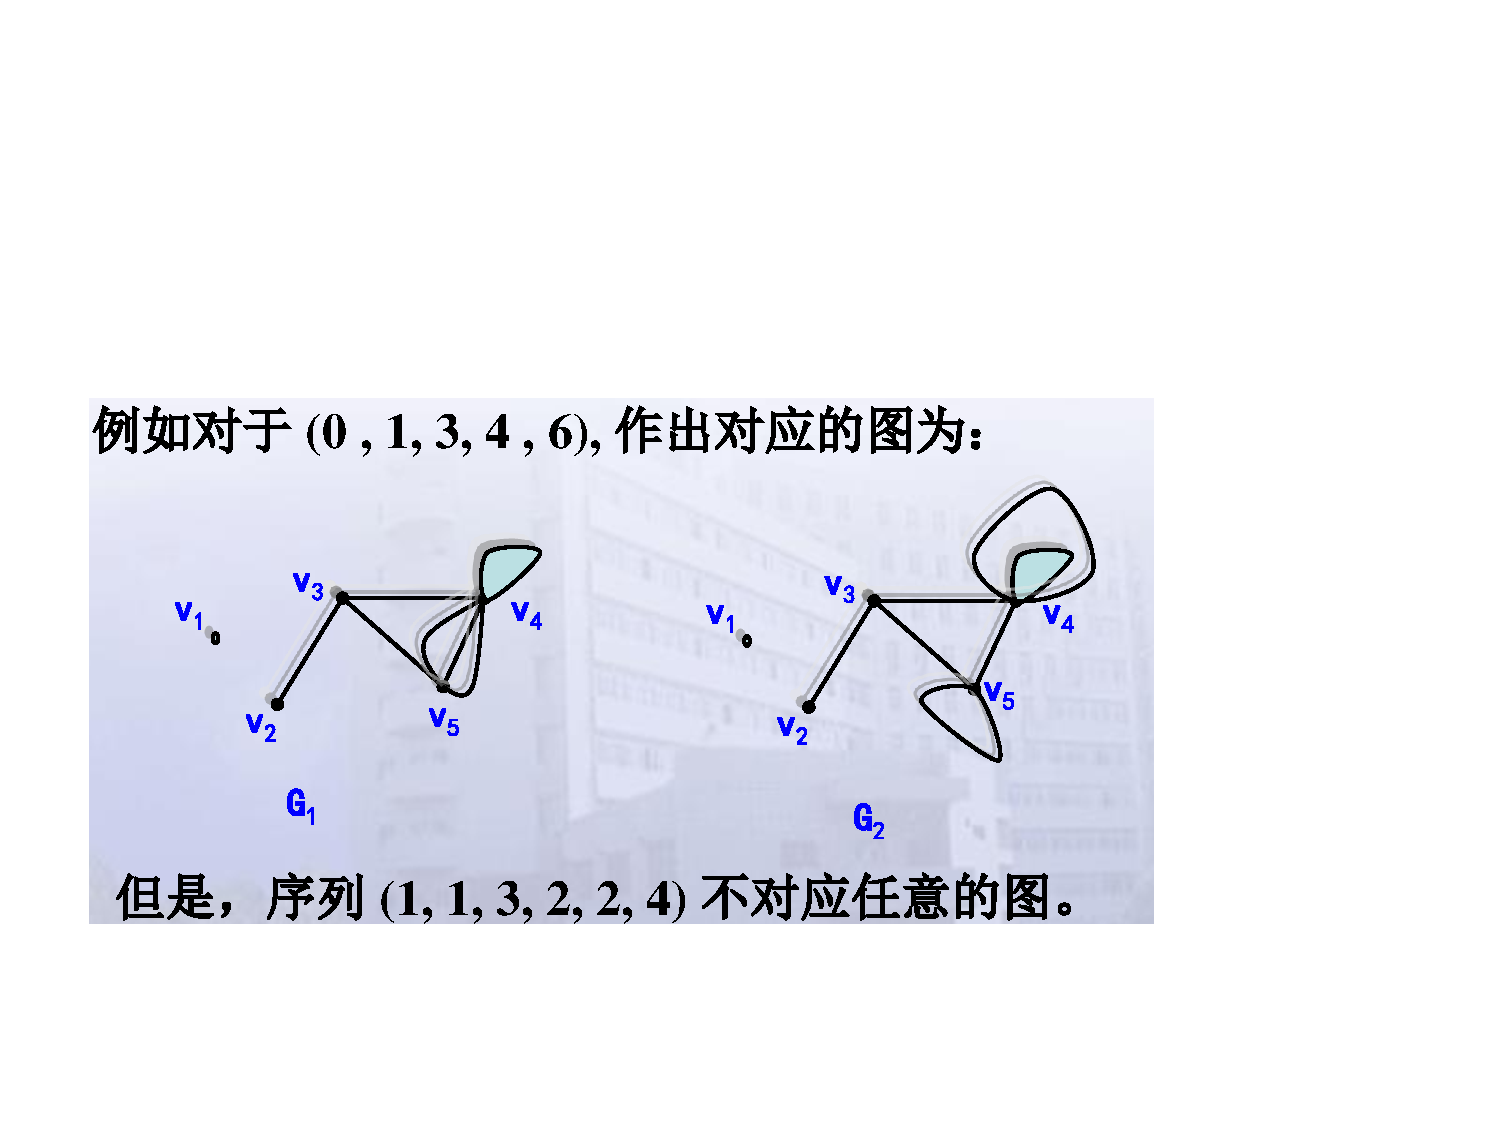
\includegraphics[scale=0.5]{image/duxulie.pdf}  
	%\caption{信息包结构} 
	\label{fig1k}  
\end{figure}


\noindent {\bfseries \textcolor{ecolor}{图序列及其性质:}}

研究一个非负整数序列是否对应简单图的问题.
\begin{definition}[图序列]
一个非负整数组如果是某简单图的度序列,我们称它为可图序列,简称图序列.
\end{definition}

\begin{theorem}
	非负整数组
	\[
	\colorbox{yellow}{$\pi=(d_1, d_2,\cdots, d_n), d_1\geq d_2 \geq \cdots \geq d_n, \sum\limits d_i = 2m$}
	\]
	是图序列的\textcolor{red}{充分条件}是:
	\[
	\colorbox{yellow}{$\pi_1=(d_2-1, d_3-1,\cdots, d_{d_1+1}-1, d_{d_1+2}, \cdots, d_n)$}
	\]是图序列.
\end{theorem}

\begin{theorem}[厄多斯1960]
	非负整数组
	\[
	\colorbox{yellow}{$\pi=(d_1, d_2,\cdots, d_n), d_1\geq d_2 \geq \cdots \geq d_n, \sum\limits d_i = 2m$}
	\]
	是图序列的\textcolor{red}{充分条件}是:
	\[
	\colorbox{yellow}{$\sum\limits_{i=1}^r d_i \leq r(r-1)+ \sum \limits_{i=r+1}^n \min\{r,d_i\}, 1 \leq r \leq n-1$}
	\]是图序列.
\end{theorem}
\begin{note}
	该定理只能做判定,证明困难.
\end{note}


\noindent {\bfseries \textcolor{ecolor}{图的频序列及其性质:}}
\begin{definition}[频序列]
设$n$阶图$G$的各点的度取$s$个不同的非负整数
$d_1,d_2,\cdots, d_s$.又设度为$d_i$的点有$b_i$个 ($i = 1,2,\cdots,s$),则
\[
\colorbox{yellow}{$\sum\limits_{i=1}^{s}b_i=n$}
\]
故非整数组($b_1,b_2,\cdots, b_s$)是n的一个划分,称为$G$的频
序列.
\end{definition}
\begin{theorem}
一个简单图$G$的n个点的度不能互不相同.
\end{theorem}
\begin{proof}
因为图G为简单图,所以:$\varDelta(G)\leq n-1$.
\begin{itemize}
	\item 情形1:若$G$没有孤立点,则$1\leq d(v) \leq n-1, \forall v\in V(G)$;
	由鸽笼原理:必有两顶点度数相同;
	\item 情形2:若$G$只有一个孤立点,设$G_1$表示$G$去掉孤立点后的部分,则$1\leq d(v) \leq n-2, \forall v\in V(G_1)$;由鸽笼原理:必有两顶点度数相同;
	\item 情形3: 若G只有两个以上的孤立点,则定理显然成立.
\end{itemize}
\end{proof}
\begin{theorem}
一个n阶图G和它的补图有相同的频序列$(n\geq 2)$.
\end{theorem}
\begin{proof}
设图$G$的任一顶点$v$的度数为$k$,则该顶点在补图中的度数为$n-1-k$.因此:在$G$中有$b$个度数为$k$的顶点,则在补图中就有$b$个度数为$n-1-k$个顶点.
\end{proof}



\subsection{子图与图的运算}
\subsubsection{子图的相关概念}
\noindent {\bfseries \textcolor{ecolor}{子图的定义:}}
\begin{definition}[子图]
	如果$V(H)\subseteq V(G), E(H)\subseteq E(G)$,且$H$中边的重数不超过$G$中对应边的条数,则称$H$为$G$的子图,记为$H\subseteq G$.特别地,当$H\subseteq G, H\ne G$时,称$H$是$G$的真子图,记为$H \subset G$.
\end{definition}

\noindent {\bfseries \textcolor{ecolor}{点与边的导出子图:}}
\begin{definition}[顶点导出子图]
	如果$V^{'}\subseteq V(G)$,则以$V^{'}$为顶点集,以两个端点均在$V^{'}$中的边集组成的图,称为图$G$的点导出子图。记为:$G[V^{'}]$.
\end{definition}


\begin{definition}[边导出子图]
	如果\colorbox{yellow}{$E^{'}\subseteq E(G)$},则以\colorbox{yellow}{$E^{'}$}为顶点集,以两个端点均在\colorbox{yellow}{$E^{'}$}中的边集组成的图,称为图$G$的边导出子图。记为:\colorbox{yellow}{$G[E^{'}]$}.
\end{definition}

\noindent {\bfseries \textcolor{ecolor}{图的生成子图:}}
\begin{definition}[生成子图]
如果图$G$的一个子图\textcolor{red}{包含$G$的所有顶点},称该子图为$G$的一个生成子图.
\end{definition}
\begin{theorem}
	\colorbox{yellow}{简单图$G=(n, m)$的所有生成子图个数为$2^{m}$}.
\end{theorem}

\subsubsection{图运算}
在图论中,将两个或更多的图按照某种方式合并,或者对一个图作某种形式的操作,可以得到很有意义的新图。将图合并或对一个图进行操作,称为图运算。

\begin{enumerate}
\item 图的删点运算
	
设\colorbox{yellow}{$V^{'}\subseteq V(G)$},在$G$中删去中的顶点和$G$中与之关联的所有边的操作,称为删点运算。记为\colorbox{yellow}{$G-V^{'}$}.特别地,如果只删去一个点$v$,则记为$G-v$.

\item 图的删边运算
	
设\colorbox{yellow}{$E^{'}\subseteq E(G)$},在$G$中删去中的顶点和$G$中的所有边的操作,称为删边运算。记为\colorbox{yellow}{$G-E^{'}$}.特别地,如果只删去一个边$e$,则记为$G-e$.
\begin{note}
 \textcolor{red}{删点要删关联的边,删边不删关联的点!}
\end{note}

\item 图的并运算

设$G_1,G_2$是$G$的两个子图,$G_1$与$G_2$并是指由$V(G_1)\cup  V(G_2)$为顶点集,以$E(G_1)\cup  E(G_2)$为边集组成的子图.记为\colorbox{yellow}{$G_1\cup G_2$}.特别地,如果$G_1,G_2$不相交(没有公共顶点),称它们的并为直接并,可以记为:\colorbox{yellow}{$G_1+ G_2$}.

\item 图的交运算

设$G_1,G_2$是$G$的两个子图,$G_1$与$G_2$交是指由$V(G_1)\cap  V(G_2)$为顶点集,以$E(G_1)\cap  E(G_2)$为边集组成的子图.记为\colorbox{yellow}{$G_1\cap G_2$}.

\item 图的差运算

设$G_1,G_2$是两个图,$G_1$与$G_2$的差是指从$G_1$中删去$G_2$中的边得到的新图。记为$G_1-G_2$.

\item 图的对称差运算(或环和运算)

设$G_1,G_2$是两个图,$G_1$与$G_2$的对称差定义为:
\[
\colorbox{yellow}{$G_1\Delta G_2 = (G_1\cup G_2) - (G_1\cap G_2) $}
\]

\item 图的联运算

设$G_1,G_2$是两个不相交的图,作$G_1+G_2$,并且将$G_1$中每个顶点和$G_2$
中的每个顶点连接,这样得到的新图称为$G_1$与$G_2$的联图。记为:\colorbox{yellow}{$G_1\lor G_2 $}. \textcolor{red}{$n=n_1+n_2, m=m_1+m_2+n_1n_2$}

\item 图的积图

设\colorbox{yellow}{$G_1=(V_1,E_1),G_2=(V_2,E_2)$},是两个图。对点集\colorbox{yellow}{$V=V_1\times V_2$}的任意两个点$u=(u_1, u_2)$与$v=(v_1, v_2)$,当$(u_1=v_1\mbox{和}u_2\mathrm{adj}v_2$或$(u_2=v_2\mbox{和}u_1\mathrm{adj}v_1$时,把$u$与$v$连接.如此得到的新图称为$G_1$和$G_2$的积图.记为:\colorbox{yellow}{$G=G_1\times G_2$}. \textcolor{red}{$n=n_1n_2, m=n_1m_2+n_2m_1$}
\begin{figure}[H]
	\small
	\centering 
	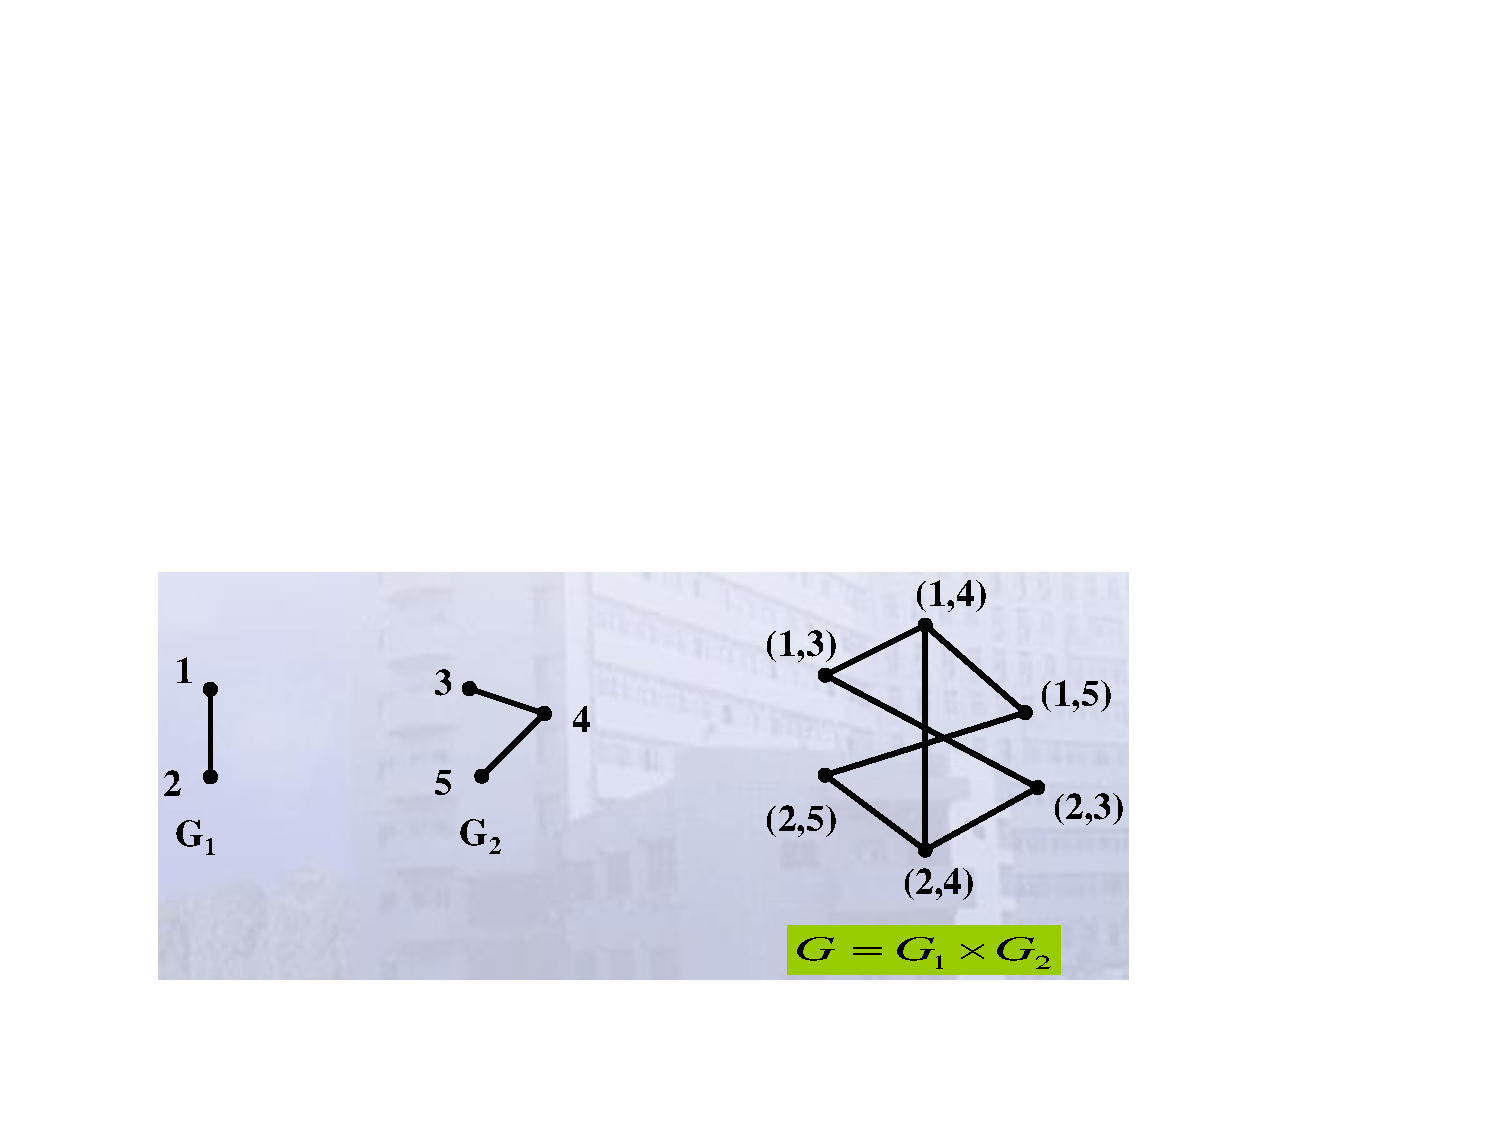
\includegraphics[scale=0.7]{image/CH1_jitu.pdf}  
	%\caption{信息包结构} 
	\label{figkk1k}  
\end{figure}
\begin{note}
	\textcolor{red}{超立方体} 
	
	{\bfseries n方体}$Q_n$: \colorbox{yellow}{$Q_1=K_2, Q_2=K_2\times K_2, \cdots, Q_n=K_2\times Q_{n-1}$}. $Q_n$有$2^n$个点,用$a_1a_2\cdots a_n$来标定,$a_i$是$0$或$1$. 如果$Q_n$两个点的二进制表示只有一位不同,则这两个点邻接. \textcolor{red}{$Q_n(n>1)$是偶图}
\end{note}
\item 图的合成图

设\colorbox{yellow}{$G_1=(V_1,E_1),G_2=(V_2,E_2)$},是两个图。对点集\colorbox{yellow}{$V=V_1\times V_2$}的任意两个点$u=(u_1, u_2)$与$v=(v_1, v_2)$,当$u_1\mathrm{adj}v_1$或$(u_1=v_1\mbox{和}u_2\mathrm{adj}v_2$时,把$u$与$v$连接.如此得到的新图称为$G_1$和$G_2$的合成图.记为:\colorbox{yellow}{$G=G_1[G_2]$}
\begin{figure}[H]
	\small
	\centering 
	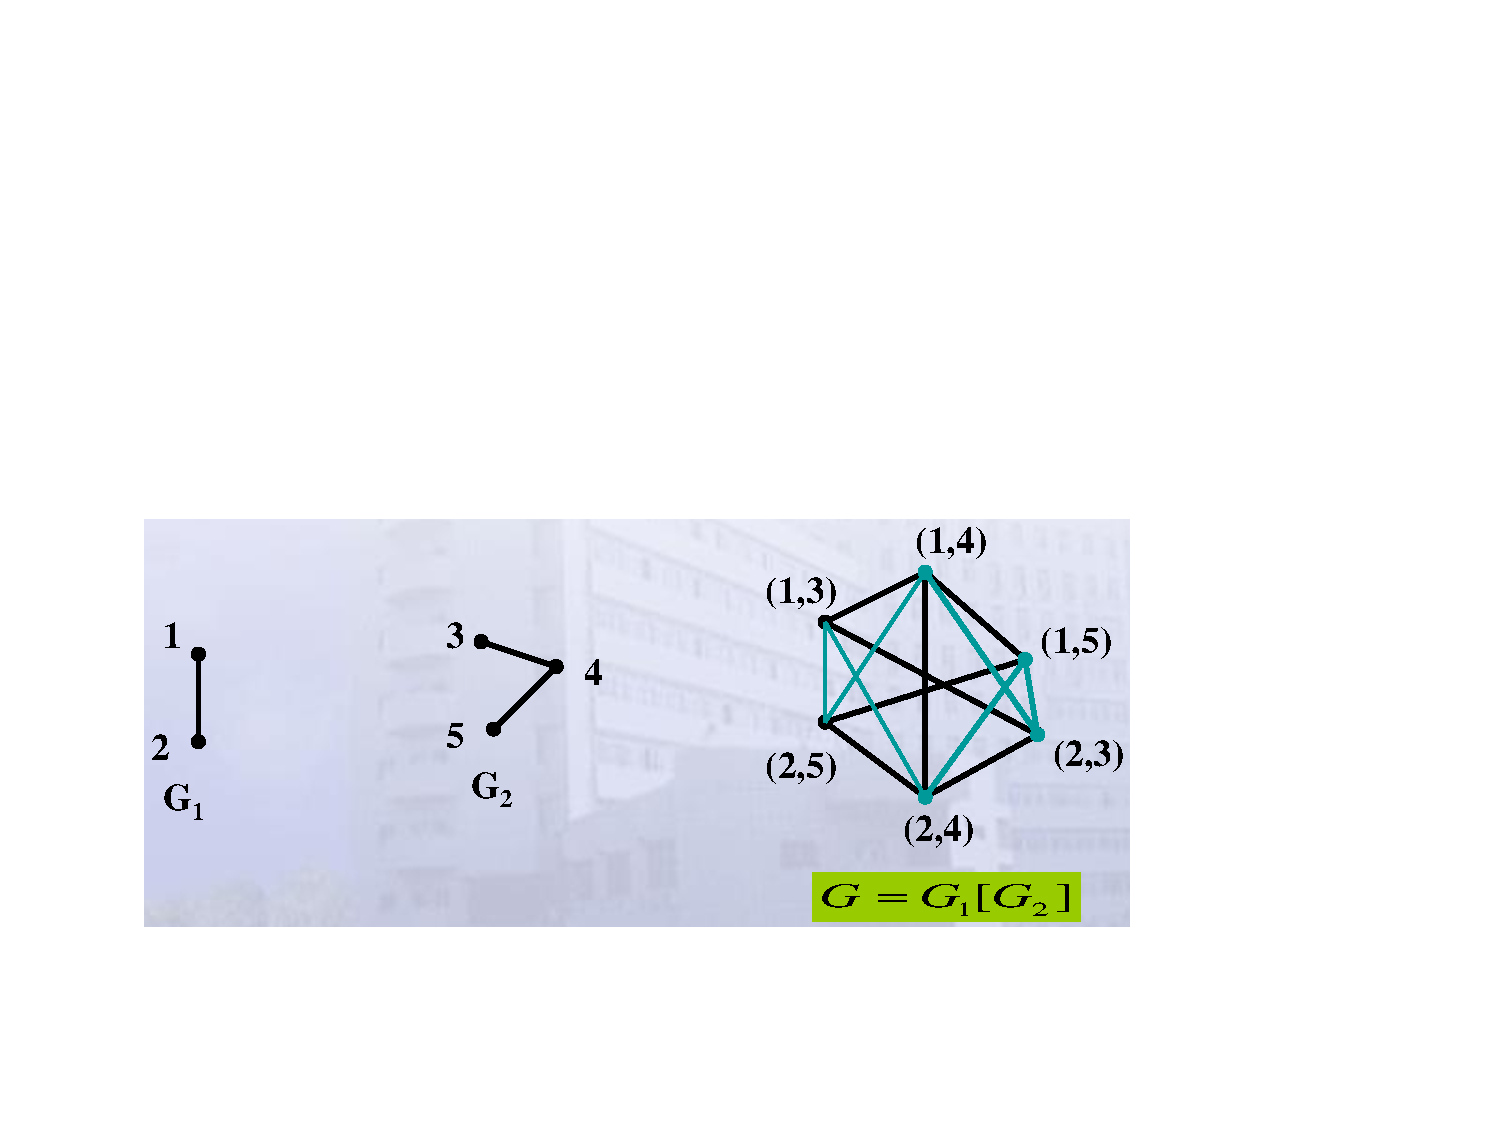
\includegraphics[scale=0.7]{image/CH1_hechengtu.pdf}  
	%\caption{信息包结构} 
	\label{figk1k}  
\end{figure}
\end{enumerate}


\subsection{路与图的连通性}
\subsubsection{路与圈相关概念}

\begin{enumerate}
\item 图中的途径:指一个有限非空序列,顶点和边交替。 \textcolor{red}{途径中边数称为途径的长度};$v_0,v_k$分别称为途径的起点与终点,其余顶点称为途径的内部点.

\item \colorbox{yellow}{\textcolor{red}{图中的迹}}:\textcolor{red}{边不重复的途径称为图的一条迹}.
\item \colorbox{yellow}{\textcolor{red}{图中的路}}: \textcolor{red}{顶点不重复的途径称为图的一条路}.
\end{enumerate}
\begin{note}
	\begin{itemize}
		\item 路是途径,也是迹,迹是途径;
		\item \textcolor{red}{起点与终点重合的途径、迹、路分别称为图的闭途径、闭迹与圈。闭迹也称为回路}.长度为k的圈称为k圈,k为奇数时称为奇圈,k为偶数时称为偶圈.
	\end{itemize}
\end{note}

\subsubsection{连通性的相关概念}

\begin{enumerate}
	\item \colorbox{yellow}{\textcolor{red}{图中两顶点的距离}}:图中顶点$u$与$v$的距离:$u$与$v$间最短路的长度称为$u$与$v$间距离。记为$d(u, v)$,如果$u$与$v$间不存在路,定义$d(u, v)=\infty$.
	\item \colorbox{yellow}{\textcolor{red}{图中两顶点的连通性}}:如果在$G$中存在$(u,v)$路,则规定$u$和$v$是连通的.
	\item  \colorbox{yellow}{\textcolor{red}{连通图}}: 如果对$G$中每一对顶点$u,v$都有一条$(u,v)$路,则称$G$为\textcolor{red}{连通图},否则称为\textcolor{red}{非连通图}.
	
	\item  \colorbox{yellow}{\textcolor{red}{连通分支}}:非连通图中每一个极大连通部分,称为G的连通分支。G的连通分支的个数,称为G的分支数,记为\colorbox{yellow}{$\omega(G)$}.
	
	\item  \colorbox{yellow}{\textcolor{red}{图的直径}}:连通图G的直径定义为:
	\[
	\colorbox{yellow}{$d(G) = \mathrm{max}\{d(u,v) |u,v \in V(G)\}$}
	\]
	如果G不连通,图G的直径定义为\colorbox{yellow}{$d(G) = \infty$}.
	.
\end{enumerate}

\subsubsection{连通性性质}

\begin{theorem}
	若图$G$不连通,则其补图连通.
\end{theorem}
\begin{proof}
如果$u, v$属于$G$的同一分支,设$w$是与$u, v$ 处于不同分支中的点,则在$G$的补图中,$u$与$w$, $v$与$w$分别邻接,于是,$u$与$v$在$G$的补图中是连通的。
	
如果$u$与$v$在$G$的两个不同分支中,则在$G$的补图中必然邻接,因此,也连通。
\end{proof}


\subsubsection{偶图的判定定理}
\begin{theorem}
	\colorbox{yellow}{\textcolor{red}{一个图是偶图当且当它不包含奇圈}}
\end{theorem}
\begin{proof}
	略.
\end{proof}

\subsection{图的代数表示}
\subsubsection{图的邻接矩阵}

\begin{definition}
设$G$为$n$阶图,$V=\{v_1, v_2, \cdots, v_n\}$,邻阶矩阵$A(G)=(a_{ij})$,
其中\textcolor{red}{$a_{ij}=l$表示$v_i$与$v_j$的边数},当$l=0$时,表示$v_i$与$v_j$不邻接.
\end{definition}
\noindent {\bfseries \textcolor{ecolor}{性质:}}

\begin{enumerate}
\item 非负性与对称性.
\item 同一图的不同形式的邻接矩阵是相似矩阵.
\item \textcolor{red}{如果$G$为简单图,则$A(G)$为布尔矩阵;行和$($列和$)$等于对应顶点的度数;矩阵元素总和为图的总度数,也就是$G$的边数的2倍}.
\item $G$连通的充分必要条件是:$A(G)$不能与如下矩阵相似:
\[	
\colorbox{yellow}{$
\begin{pmatrix}
	A_{11}& O\\
	O&A_{22}\\
\end{pmatrix}
$}
\]
\begin{proof}
	略.
\end{proof}
\begin{note}
\textcolor{red}{非连通图的邻接矩阵一定能够写成准对角矩阵形式}.
\end{note}
\item 

\begin{theorem}
	设\colorbox{yellow}{$A^{k}(G) = (a_{ij}^{(k)}) $},则$a_{ij}^{(k)}$表示顶点$v_i$到$v_j$的途径长度为$k$的途径条数.
\end{theorem}
\begin{proof}
略.
\end{proof}
\begin{corollary}
设$A$为简单图$G$的邻接矩阵,则:\textcolor{red}{$A^2$的元素$a_{ii}^{(2)}$是$v_i$的度数},$A^3$的元素$a_{ii}^{(3)}$是含$v_i$的三角形个数的2倍数
\end{corollary}
\end{enumerate}

\subsubsection{图的关联矩阵}
\begin{definition}
	设$G$是$(n,m)$阶图.定义$G$的关联矩阵:\colorbox{yellow}{$M(G)=(a_{ij})_{(n\times m)}$}
	
	其中:\colorbox{yellow}{$a_{ij}=l, \quad l$表示$v_i$和$e_j$关联的次数(0,1,或2(环))}
\end{definition}
\noindent {\bfseries \textcolor{ecolor}{性质:}}
\begin{enumerate}
	\item 关联矩阵的元素为0,1或2;
	\item \textcolor{red}{关联矩阵的每列和为2;每行的和为对应顶点度数}.
\end{enumerate}

\subsubsection{图的邻接谱}
\begin{theorem}
	设$A(G)$的谱为$Spec A(G)=\begin{pmatrix}
		\lambda_1 &\lambda_2&\cdots & \lambda_n\\
		m_1&m_2&\cdots & m_n
	\end{pmatrix}$,则
\[
\sum\limits_{i=1}^{s}m_i\lambda_i^2=2m
\]其中$m_i$是特征值$\lambda_i$的重数,$m$为$G$的边数.
\end{theorem}
\begin{note}
	图$G$邻接矩阵$A$所有特征值的平方和为图$G$边数的2倍.
\end{note}
\begin{example}
	若$G=K_n$,则$Spec A(K_n)=\begin{pmatrix}
		-1 &n-1\\
		n-1&1
	\end{pmatrix}$.
\end{example}
\begin{note}
$K_n$的最大特征值为$n-1$.	
\end{note}


\subsection{最短路及其算法}
\subsubsection{几个相关概念}
\begin{enumerate}
	\item \colorbox{yellow}{\textcolor{red}{边赋权图}}:在图$G$的每条边$e$上赋予一个实数$\omega(e)$后, 称$G$为边赋权图。
	\item \colorbox{yellow}{\textcolor{red}{边赋权图中的最短路}}:设$G$为边赋权图, $u$与$v$是$G$中两点,在连接$u$与$v$的所有路中,路中各边权值之和最小的路,称为$u$与$v$间的最短路.
\end{enumerate}

\subsubsection{最短路算法}
\begin{note}
	主要考填空题,肉眼目测最短路.
\end{note}

\subsection{极图}
\begin{definition}
	\begin{enumerate}
		\item 若简单图$G$的点集$V$有一个划分:$V=\bigcup\limits_{i=1}^{l} V_{i}, V_{i} \cap V_{j}=\phi, i \neq j$,且所有的$V_i$非空,$V_i$内的点均不邻接,称$G$是一个$l$ 部图.
		\item 如果在一个$l$ 部图$G$中,任意部$V_i$中的每个顶点同$G$中其
		它各部中的每个顶点均邻接,称$G$为\colorbox{yellow}{\textcolor{red}{完全$l$部图}}. 记作:$G=K_{n_1,n_2,\cdots,n_l}(n_i=|V_i|, 1\leq i \leq  n)$. 显然\colorbox{yellow}{$|V|=\sum\limits_{i=1}^{l}n_i$}和\colorbox{yellow}{$m(G)=\sum\limits_{1\leq i < j \leq l}n_in_j$}.
	\end{enumerate}
\end{definition}

\begin{theorem}
	$n$阶完全偶图$K_{n_1,n_2}$的边数$m=n_1n_2$,且有$m\leq \left[\frac{n^2}{4}\right]$.
\end{theorem}
\begin{proof}
	\( m=n_{1} n_{2} \) 显然. 下面证明第二结论:
	\[
	m\left(K_{n_{1}, n_{2}}\right)=m\left(K_{n-n_{2}, n_{2}}\right)=\left(n-n_{2}\right) n_{2}=\frac{n^{2}}{4}-\left(\frac{n}{2}-n_{2}\right)^{2} \leq\left\lfloor\frac{n^{2}}{4}\right\rfloor
	\]
\end{proof}

\begin{definition}
	如果在一个 \( {n} \) 个点的完全 \( {l} \) 部图 \( {G} \) 中有:
	\[
	\begin{split}
		 &n=k l+r, 0 \leq r<l,\\
		 &\left|V_{1}\right|=\left|V_{2}\right|=\cdots=\left|V_{r}\right|=k+1,\\
		 & \left|V_{r+1}\right|=\left|V_{r+2}\right|=\cdots=\left|V_{l}\right|=k, \\
	\end{split}
	\]
	则称 \( G \) 为 \( n \) 阶完全 \( l \) 几乎等部图, 记为 \( T_{l, n} \).所有$l$部顶点数相等,\( n \)阶完全 \( l \) 几乎等部图称为,\( n \)阶完全\( l \)等部图.
\end{definition}


\begin{theorem}
	$n$阶$l$部图$G$有最多边数的充要条件是$G \cong  T_{l, n}$.
\end{theorem}



\subsubsection{托兰定理}

\begin{theorem}
	若$G$度弱于$H$,一定有$m(G)\leq m(H)$.
\end{theorem}
\begin{note}
	反过来不一定,因为两个图可能不存在度弱关系.
\end{note}
\begin{theorem}
	若$n$阶简单图$G$不包含$K_{l+1}$,则$G$度弱于某个完全 $l$
	部图$H$,且若$G$具有与 $H$ 相同的度序列,则$G \cong H$.
\end{theorem}
\begin{theorem}[托兰定理]
	若$n$阶简单图$G$不包含$K_{l+1}$,则:
	\[
	m(G)\leq m(T_{l, n})
	\]
	仅当$G \cong  T_{l, n}$时,有$m(G)= m(T_{l, n})$.
\end{theorem}

\begin{theorem}
$n$ 阶简单图$G$不包含$K_{l+1}$,则$m(T_{l, n})=C_{l}^{2}\left(\dfrac{n}{l}\right)^2$
% G m\left(T_{l, n}\right)=C_{l}^{2}\left(\frac{n}{l}\right)^{2} \text {. }
\end{theorem}
\begin{example}
	
	\begin{enumerate}
		\item $n$ 阶简单图 $G$不包含$K_3$, 则 $G$ 最多有 $\frac{n^2}{4}$条边.
		\item $9$ 阶简单图 $G$不包含$K_4$, 则 $G$ 最多有$27$条边.
	\end{enumerate}
\end{example}











